\documentclass{siproblemset}

% SI Session Information
\course{MTH 1321}       % the course of your SI
\sessionnum{18}         % (optional) specify the session number
\sessiondate{11/6/19}   % the date of the session

\warmup{Concept Review}
\topic{Applied Optimization}
\topic{Trigonometric Optimization}
\cooldown{Finding the Objective Function}

% Worksheet Information
\title{Applied Optimization}
\sections{Section 4.7}
\withnamespace

\begin{document}
    \maketitle
    
    \activity{Warmup}{Concept Review}{Work \textbf{alone} to answer these questions. Try not to use your notes.}{15 minutes}
    
    \frq{What are the steps to optimize a function?}
    \Largesp
    \mcq{When making a sign diagram for the derivative of a function, what x-values do we need to put on the number line?}{
        \task 
        \tinysp
        \task
        \tinysp
        \task
        \tinysp
    }
    \newpage
    
    \activity{Activity 1}{Optimization}{Make a \textbf{group of two or three, all with the same colored worksheets}, to work together to answer your assigned question. Then, try to answer the other question. Try not to use your notes. \textbf{DO NOT use a calculator}.}{30 minutes}
    
    \mcq{Your task is to design a rectangular industrial warehouse consisting of three separate spaces of equal size as in the figure below. The wall materials cost \$500 per linear meter and your company allocates \$2,400,000 for that part of the project involving the walls.}{
        \task Which dimensions maximize the area of the warehouse?
        \task What is the area of each compartment in this case?
    }
    \begin{center}
        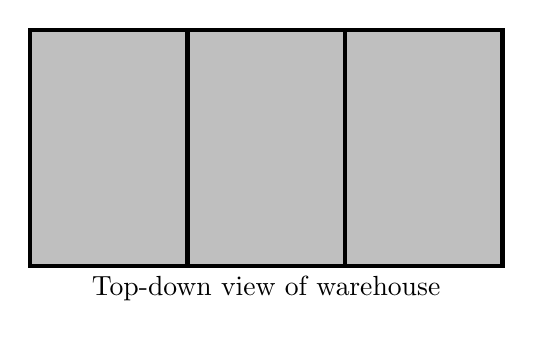
\begin{tikzpicture}
            \filldraw[fill=lightgray] (0,0) rectangle (6,3);
            \draw[black, ultra thick, line cap=rect] (0,0) -- (6,0);
            \node at (3,0) [below,align=center]{Top-down view of warehouse};
            \draw[black, ultra thick, line cap=rect] (0,3) -- (6,3);
            \draw[black, ultra thick] (0,0) -- (0,3);
            \draw[black, ultra thick] (2,0) -- (2,3);
            \draw[black, ultra thick] (4,0) -- (4,3);
            \draw[black, ultra thick] (6,0) -- (6,3);
        \end{tikzpicture}
    \end{center}
    \newpage
    \frq{[1.] (continued)}
    \newpage

    \activity{Activity 2}{Trigonometric Optimization}{Make a \textbf{group of two or three, all with different colored worksheets}, to answer your assigned question. Then, try to answer the other questions. Try not to use your notes. \textbf{DO NOT use a calculator}.}{30 minutes}
    
    \frq{The force $F$ (in Newtons) required to move a box of mass $m$ kg in motion by pulling on an attached rope (see the figure below) is $$F(\theta)=\frac{\mu_k m g}{\cos\theta+\mu_k\sin\theta}$$ where $\theta$ is the angle between the rope and the horizontal, $\mu_k$ is the coefficient of kinetic friction and $g=\v{9.81}$ is the acceleration due to gravity. Find the angle $\theta$ that minimizes the required force $F$, assuming that $\mu_k=0.5$.}
    \begin{center}
        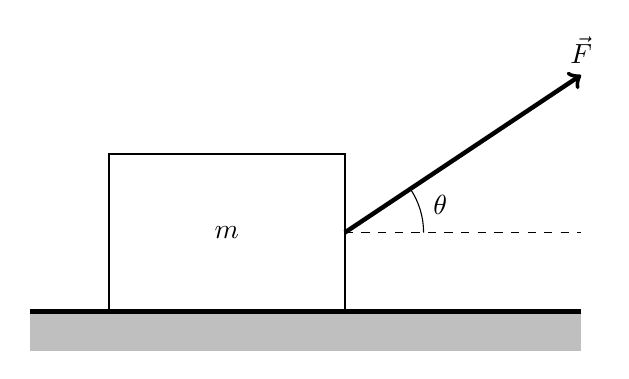
\begin{tikzpicture}
            \fill[fill=lightgray] (-1,0) rectangle (6,-0.5);
            \draw[ultra thick] (-1,0) -- (6,0);
            \draw[thick] (0,0) rectangle (3,2) node[midway]{$m$};
            \draw[->,ultra thick] (3,1) -- (6,3) node[above]{$\vec F$};
            \draw[dashed] (3,1) -- (6,1);
            \draw (4,1) arc (0:34:1);
            \node at (4,1.6) [below right]{$\theta$};
        \end{tikzpicture}
    \end{center}
    \newpage
    \frq{[1.] (continued)}
    \newpage
    \activity{Cooldown}{Finding the Objective Function}{Work \textbf{as a class} to answer these questions. Try not to use your notes.}{15 minutes}
    
    \mcq{For each scenario below, find the objective/key function.}{
        \task Find two positive numbers such that their product is 192 and the sum of the first plus three times the second is as small as possible.
        \Smallsp
        \task Find the dimensions of the rectangle of maximum area that can be inscribed in a circle of radius $\SI{4}{\meter}$.
        \Smallsp
        \task A \SI{5}{\meter} piece of string is bent into an L-shape. Where should the bend be made to minimize the distance between the two ends?
        \Smallsp
        \task A rancher will use 600 feet of fencing to build a corral in the shape of a semicircle on top of a rectangle. Find the dimensions that maximize the area of the corral.
    }
\end{document}